% ============================================================================
\section{Introduction and overview}
% ============================================================================

\begin{frame}{Introducing the speech recognition task}
  \begin{itemize}
    \item \textbf{Broad goal.} Given audio, produce exact transcript of words from speaker(s).
    \item \textbf{Verbatim (Exact) Transcription:} Capturing every ``um,'' word fragment, repetition, and disfluency to preserve the true speech signal.
    \item \textbf{Clean (Readable) Transcripts:} Text that omits or normalizes minor speech errors and filler words, yielding more fluent, reader-friendly output.
    \item \textbf{Real-Time, Low-Latency Operation:} For interactive settings (voice assistants, live captions), ASR must process audio as it arrives. Keep end-to-end latency under 200 ms for natural dialogue flow.
    \item \textbf{On-Device and Edge Constraints:} Need to run ASR on devices with no cloud support. Compute and memory may be limited.
  \end{itemize}
  \vspace{0.5em}
  
  \footnotesize\href{https://web.stanford.edu/class/cs224s/semesters/2025-spring/lecture-slides/switchboard_example.pdf}{Switchboard corpus} conversation example
\end{frame}

% --- Stanford CS224S lec9, slide 44 ---
\begin{frame}{Arc of Recent History}
  \begin{itemize}
    \item \textbf{In 2010:}
    \begin{itemize}
      \item ASR, TTS, dialog all used specialized, hard-to-build modeling approaches
      \item Industry application of SLU systems limited. ASR ``didn't quite work well enough''
    \end{itemize}
    \item \textbf{Today:}
    \begin{itemize}
      \item ASR, TTS, dialog all use deep learning approaches. Less specialized and better performance
      \item Spoken language systems are everywhere!
      \item New tools enable building full systems
    \end{itemize}
  \end{itemize}
\end{frame}

% --- Stanford CS224S lec9, slide 45 ---
\begin{frame}{History: Foundational Insights 1900s--1950s}
  \textbf{Automaton:}
  \begin{itemize}
    \item Markov 1911
    \item Turing 1936
    \item McCulloch-Pitts neuron (1943)
    \begin{itemize}
      \item \href{http://mar.bsee.swin.edu.au/cht/net204/lecture10/ann/node1.html}{mar.bsee.swin.edu.au/cht/net204/lecture10/ann/node1.html}
      \item \href{http://www.epfl.ch/mtap/tutorial/english/mcpitts.html}{www.epfl.ch/mtap/tutorial/english/mcpitts.html}
    \end{itemize}
    \item Shannon (1948) link between automata and Markov models
  \end{itemize}
  \textbf{Human speech processing}
  \begin{itemize}
    \item Fletcher at Bell Labs (1920's)
  \end{itemize}
  \textbf{Probabilistic/Information-theoretic models}
  \begin{itemize}
    \item Shannon (1948)
  \end{itemize}
\end{frame}

% --- Stanford CS224S lec9, slide 46 ---
\begin{frame}{Early Recognition: 1920's Radio Rex}
  \begin{columns}
    \column{0.42\textwidth}
    \centering
    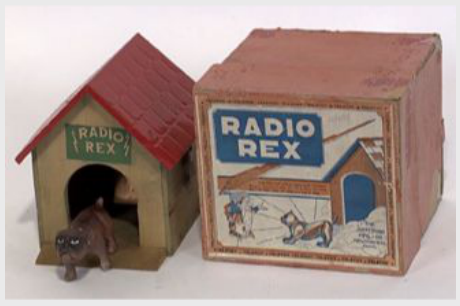
\includegraphics[width=0.95\textwidth]{assets/New-Lecture-STT/cs224s_lec9_slide_46.png} \\
    \vspace{0.5em}
    \scriptsize\textit{Radio Rex toy and box (c. 1920s)}
    \column{0.56\textwidth}
    \textbf{1920's Radio Rex}
    \begin{itemize}
      \item Celluloid dog with iron base held within house by electromagnet against force of spring
      \item Current to magnet flowed through bridge which was sensitive to energy at 500 Hz
      \item 500 Hz energy caused bridge to vibrate, interrupting current, making dog spring forward
      \item The sound ``e'' (ARPAbet [eh]) in Rex has 500 Hz component
    \end{itemize}
  \end{columns}
\end{frame}

% --- Stanford CS224S lec9, slide 47 ---
\begin{frame}{ASR: 1950's -- Early Speech Recognizers}
  \begin{itemize}
    \item \textbf{1952: Bell Labs single-speaker digit recognizer}
    \begin{itemize}
      \item Measured energy from two bands (formants)
      \item Built with analog electrical components
      \item 2\% error rate for single speaker, isolated digits
    \end{itemize}
    \item \textbf{1958:} Dudley built classifier that used continuous spectrum rather than just formants
    \item \textbf{1959:} Denes ASR combining grammar and acoustic probability
  \end{itemize}
\end{frame}

% --- Stanford CS224S lec9, slide 48 ---
\begin{frame}{ASR: 1970's and 1980's}
  \begin{itemize}
    \item \textbf{Hidden Markov Model 1972}
    \begin{itemize}
      \item Independent application of Baker (CMU) and Jelinek/Bahl/Mercer lab (IBM) following work of Baum and colleagues at IDA
    \end{itemize}
    \item \textbf{ARPA project 1971--1976}
    \begin{itemize}
      \item 5-year speech understanding project: 1000 word vocab, continuous speech, multi-speaker
      \item SDC, CMU, BBN
      \item Only 1 CMU system achieved goal
    \end{itemize}
    \item \textbf{1980's +}
    \begin{itemize}
      \item Annual ARPA ``Bakeoffs''
      \item Large corpus collection:
      \begin{itemize}
        \item[] \textcolor{red}{$\blacksquare$} TIMIT
        \item[] \textcolor{red}{$\blacksquare$} Resource Management
        \item[] \textcolor{red}{$\blacksquare$} Wall Street Journal
      \end{itemize}
    \end{itemize}
  \end{itemize}
\end{frame}

% --- Stanford CS224S lec9, slide 52 ---
\begin{frame}{Recent ASR Improvements}
  \centering
  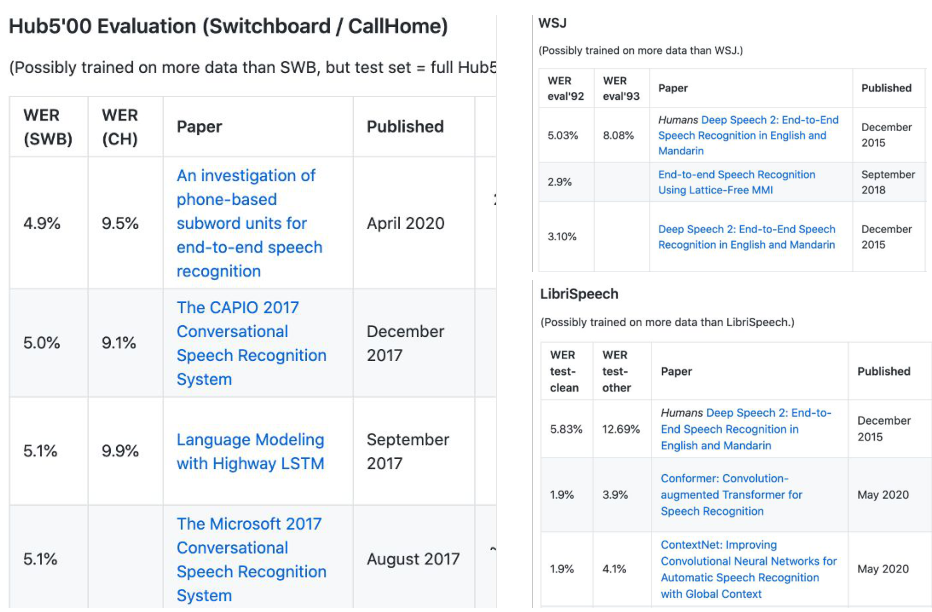
\includegraphics[width=\textwidth,height=0.92\textheight,keepaspectratio]{assets/New-Lecture-STT/cs224s_lec9_slide_52.png}
\end{frame}
